%%%%%%%%%%%%%%%%%%%%%%%%%%%%%%%%%%%%%%%%%%%%%%%%%%%%%%%%%%%%%%%%%
% Contents: The home chapter
% $Id: grisbi-manuel-home.tex, v 0.4 2002/10/27 Daniel Cartron
% $Id: grisbi-manuel-home.tex, v 0.5.0 2004/06/01 Loic Breilloux
% $Id: grisbi-manuel-home.tex, v 0.6.0 2011/11/17 Jean-Luc Duflot
% some of its content was in menus chapter:
% $Id: grisbi-manuel-menus.tex, v 0.5.0 2004/06/01 Loic Breilloux
% $Id: grisbi-manuel-home.tex, v 0.8.9 2012/04/27 Jean-Luc Duflot
% $Id: grisbi-manuel-home.tex, v 1.0 2014/02/12 Jean-Luc Duflot
%%%%%%%%%%%%%%%%%%%%%%%%%%%%%%%%%%%%%%%%%%%%%%%%%%%%%%%%%%%%%%%%%

\chapter{Eintritt in Grisbi\label{entrance}}%Entrée dans Grisbi%Entering Grisbi

\section{Auswahl einer Datei\label{select-file}}%Sélection d'un fichier%Selecting a file

\vspacepdf{3mm}			% vertical space = 5 mm

Wenn Sie die Anwendung starten, zeigt Grisbi eine Seite an, die es Ihnen ermöglicht, auf verschiedene Weise zu beginnen.%When you launch the application, Grisbi displays a page allowing you to get started in different ways.%Au lancement de l'application, Grisbi affiche la page qui vous permet de démarrer de différentes manières.

\vspacepdf{3mm}			% espace: 5 mm

Sie können das Grisbi-Fenster in \indexword{Vollbild}\index{Anzeige!Vollbild}\index{Vollbild!Anzeige} durch Drücken der Funktionstaste \key{F11} anzeigen und mit derselben Taste zurückgehen.%You can display the Grisbi window in \indexword{full screen}\index{display!full screen}\index{full screen!display} by pressing the function key \key{F11}, and go back using the same key.%Vous pouvez afficher la fenêtre de Grisbi en \indexword{plein écran}\index{affichage!plein écran}\index{plein écran!affichage} par la touche de fonction \key{F11}, et revenir en arrière par la même touche.			% "!" separates the term from the subterm of the index entry

\vspacepdf{3mm}			% espace: 5 mm

\begin{figure}[htbp]			% h=here, t=top, b=bottom, p=page of float to force the figure here, not in a next page.
	\begin{center}					% image centrée
		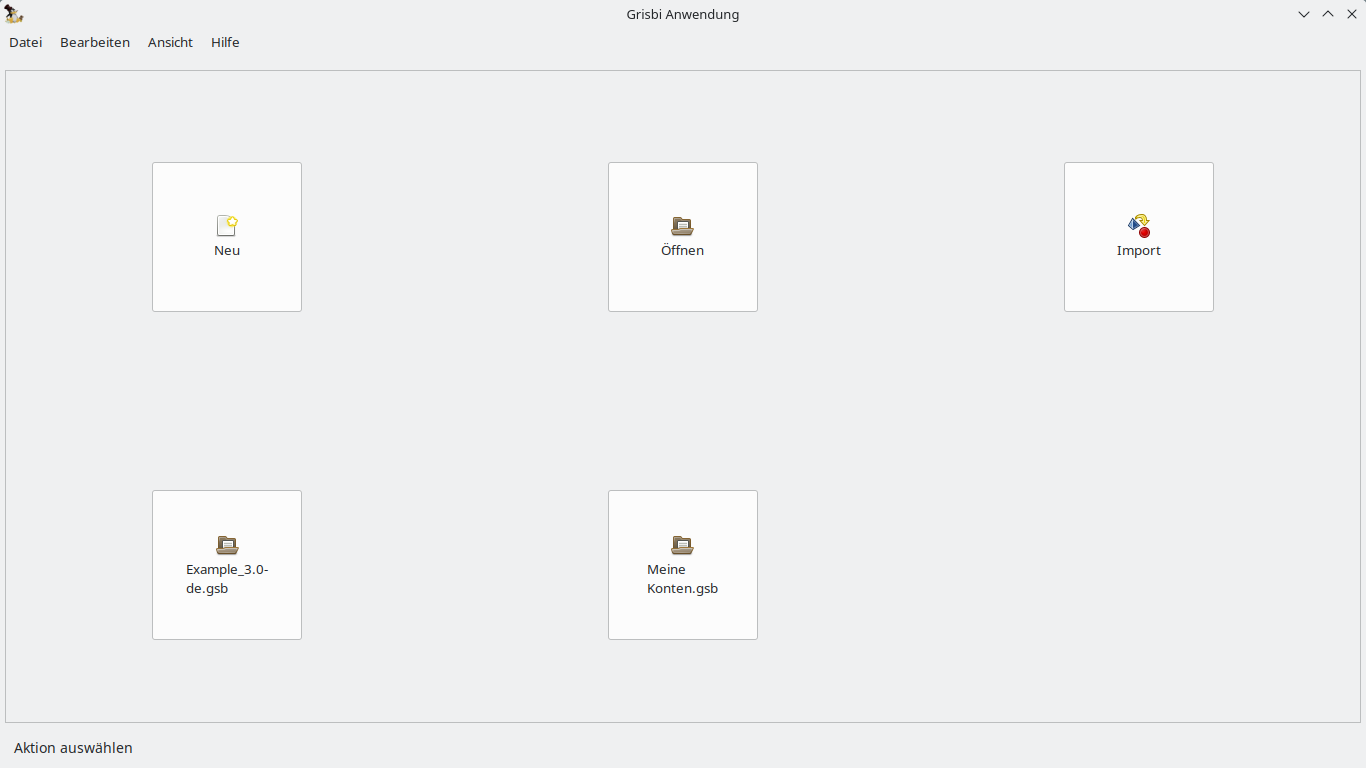
\includegraphics[width=0.95\textwidth]{image/screenshot/home_start_grisbi}		% width=95% as wide as the current text
	\end{center}
	\caption{Startfenster}%Start-up window}%Fenêtre de démarrage}			% sous-titre/subtitle
	\label{home_start_grisbi}					% figure's ref., use for link in text with \refimage{}
\end{figure}

\vspacepdf{3mm}			% espace: 5 mm

Neben der Menüleiste enthält dieses Fenster eine Reihe von Bedienfeldern:%In addition to the menu bar, this window displays a number of panels:%En plus de la barre de menu, cette fenêtre affiche plusieurs pavés:

\begin{itemize}
	\item die Schaltfläche \dequote{Neu}, um den Assistenten \dequote{Assistent für neue Datei} zu starten;%le pavé Nouveau, pour lancer l'assistant \frquote{Aide à la création d'un nouveau fichier de comptes};
	\item die Schaltfläche \dequote{Öffnen}, um einen Dateimanager anzuzeigen, mit dem Sie nach einer vorhandenen Kontendatei auf Ihrem Computer suchen können;%le pavé Ouvrir, pour afficher un gestionnaire de fichier avec lequel vous pourrez chercher un fichier de comptes existant dans votre ordinateur;
	\item die Schaltfläche {Import}, um den Assistenten {Assistent für eine neue Datei mittels Import} zu starten;%le pavé \frquote{Importer}, pour lancer l'assistant \frquote{Importation des opérations par Grisbi};
	\item eine oder mehrere weitere Schaltflächen, die nach Kontodateien benannt sind, die Grisbi bereits verwendet hat.%un ou plusieurs autres pavés, portant le nom de fichiers de comptes que Grisbi a déjà utilisés.
\end{itemize}

\vspacepdf{5mm}

\textbf{Notiz}: Schaltflächen mit den Namen von Kontodateien, die Grisbi bereits verwendet hat, sind nur vorhanden, wenn diese Dateien existieren; wenn Sie sie von dieser Eingabeseite entfernen möchten, verschieben Sie sie in ein anderes Verzeichnis oder löschen Sie sie.%les pavés portant les noms des fichiers de comptes que Grisbi a déjà utilisés ne sont présents que si ces fichiers existent; si vous voulez les enlever de cette page d'entrée, déplacez-les dans un autre répertoire, ou supprimez-les.

\vspacepdf{3mm}			% espace: 5 mm

Unten auf der Seite werden Sie durch ein Banner aufgefordert, eine Aktion auszuwählen, indem Sie eine dieser Schaltflächen wählen.%En bas de page, un bandeau vous appelle à choisir une action en sélectionnant l'un de ces pavés.

\vspacepdf{3mm}			% espace: 5 mm

Wenn Sie die Grisbi-Software nur kennenlernen möchten, um eine Vorstellung davon zu bekommen, wie sie aussieht und was sie kann, können Sie stattdessen eine Beispieldatei wie die auf der Website \lang{Sourceforge.net}\footnote{\urlSourceForgeDocumentation{}} im Ordner \dequote{examples} verwenden.%Si vous voulez juste découvrir le logiciel Grisbi pour avoir un aperçu de son aspect et de ses possibilités, vous pouvez à la place utiliser un fichier exemple comme celui présent sur le site de \lang{Sourceforge.net}\footnote{\urlSourceForgeDocumentation{}} dans le dossier \frquote{\textsf{examples}}.		% (voir la section \vref{new-example}).

\vspacepdf{5mm}			% espace: 5 mm

\textbf{Notiz}: Durch einfaches Anklicken der heruntergeladenen Beispieldatei wird Grisbi gestartet und zeigt das Home-Fenster\refimage{home_3.0} direkt an, ohne das Startfenster zu durchlaufen.%en cliquant simplement sur le fichier exemple téléchargé, Grisbi s'exécutera en affichant directement la fenêtre d'accueil\refimage{home_3.0} sans passer par la fenêtre de démarrage.

\section{Startseite\label{home}}%Homepage%Accueil

\vspacepdf{3mm}

Wenn eine Kontodatei geöffnet wird, zeigt Grisbi die Startseite\refimage{home_3.0} an.%When an account file is opened, Grisbi displays its home page\refimage{home_3.0}.%When the application starts, Grisbi displays this
Dies ist die Startseite des Programms, auf die Sie jederzeit durch Klicken auf die Registerkarte \menus{Konten} zugreifen können.%This is the start page of the programme and can be accessed at any time by clicking on the \menus{Accounts} tab.

\vspacepdf{3mm}

\begin{figure}[htbp]			% h=here, t=top, b=bottom, p=page of float to force the figure here, not in a next page.
	\begin{center}
		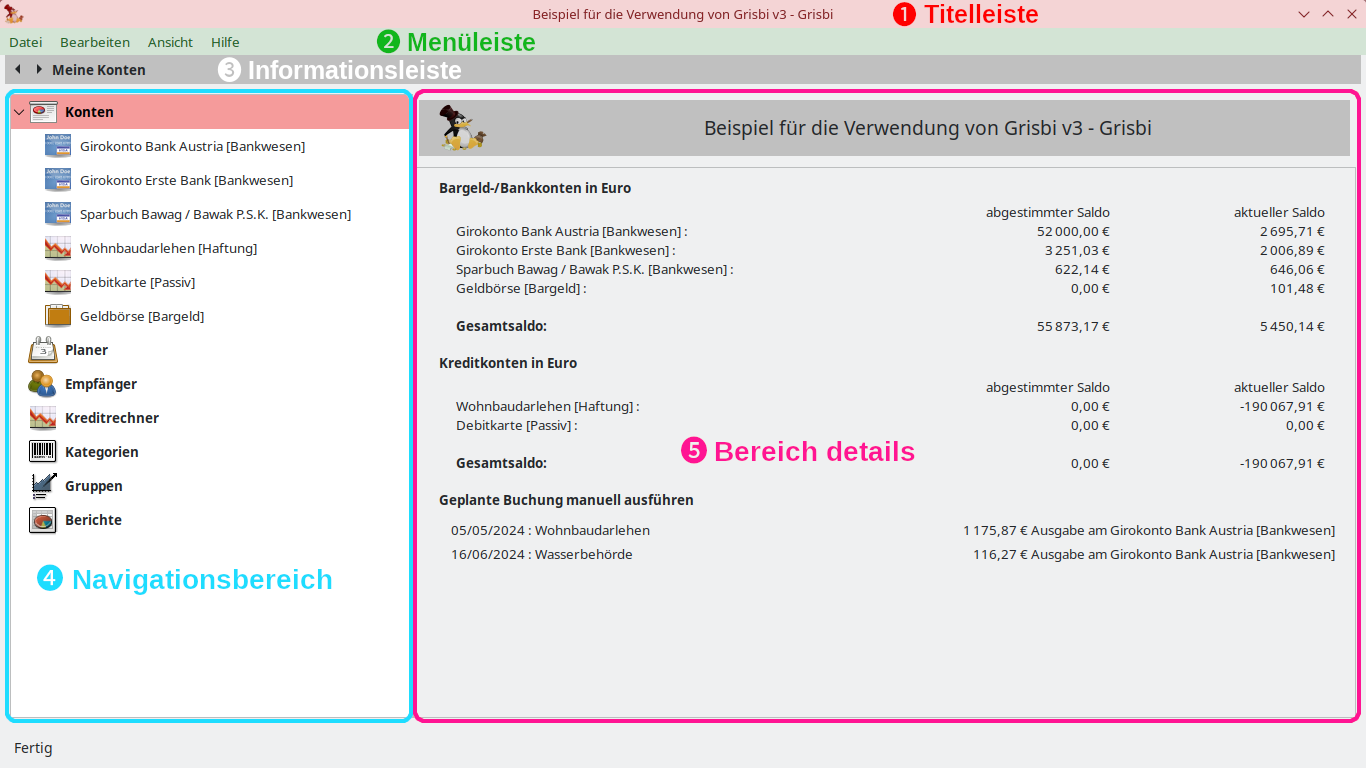
\includegraphics[width=1\textwidth]{image/screenshot/home_3.0.png}
	\end{center}
	\caption{Kontenübersichtsseite}		% sous-titre/subtitle
	\label{home_3.0}
\end{figure}

\vspacepdf{3mm}

Grisbi zeigt alle Seiten auf die gleiche Weise an: Wie jede Software zeigt sie an:%Alle Grisbi-Bildschirme haben das gleiche allgemeine Aussehen. Er zeigt eine Menüleiste, die Zugang zu den meisten wichtigen Funktionen von Grisbi bietet, sowie drei Hauptbereiche:%All Grisbi screens have the same general appearance. It displays a menu bar that gives access to most of Grisbi's important features, and three main areas:

\begin{itemize}%[\large \textcircled{\small 2}]
	\item[\large\textcircled{\small 1}] die Titelleiste;%une barre de titre;
	\item[\large\textcircled{\small 2}] die Menüleiste, die Zugang zu den meisten wichtigen Funktionen der Grisbi bietet;%une barre de menus qui donne accès à la plupart des fonctionnalités importantes de Grisbi;
\end{itemize}
sowie drei Grisbi spezifische Bereiche:%as well as three specific Grisbi zones:%et aussi trois zones qui sont spécifiques à Grisbi:
\begin{itemize}%[3,4,5]
	\item[\large\textcircled{\small 3}] die Informationsleiste unter der Menüleiste;%la barre d'information, sous la barre de menus;
	\item[\large\textcircled{\small 4}] die Navigationsbereich;%le panneau de navigation;
	\item[\large\textcircled{\small 5}] die Bereich details%le panneau des détails
\end{itemize}

\section{Informationsleiste\label{home-synthesis}}

Die Informationsleiste zeigt den Namen der aktuell ausgewählten Registerkarte an und kann ganz rechts bestimmte Bilanzen anzeigen, die sich auf das beziehen, was im Detailbereich ausgewählt wurde.%The information bar shows the name of the currently selected tab select tab di can display, completely to the right, certain balances relating to what is selected in the details panel.

\vspacepdf{5mm}

\textbf{Notiz}: die standardmäßig angezeigte Informationsleiste kann durch Deaktivieren eines Kontrollkästchens in den Einstellungen \vref{setup-display-toolbars} ausgeblendet werden.%\textbf{Note}: the information bar, displayed by default, can be hidden by unchecking a box in the preferences \vref{setup-display-toolbars}.
\vspacepdf{3mm}

Um eine der in der Navigationsleiste angezeigten Registerkarten auszuwählen, klicken Sie einmal oder mehrmals auf eines der beiden kleinen Dreiecke oben links in der Leiste.  Die angezeigten Elemente sind: \menus{Konten}, \menus{Planer}, \menus{Empfänger}, \menus{Kreditrechner}, \menus{Kategorien}, \menus{Gruppen} und \menus{Berichte}.  Wenn die Elemente \menus{Konten} und \menus{Berichte} erweitert wurden, um ihre Unterkategorien anzuzeigen, werden diese auch einzeln angezeigt.%To select one of the tabs displayed in the navigation panel click one or more times on one of the two small triangles on the top left of the panel.  The items displayed are: \menus{Accounts}, \menus{Scheduler}, \menus{Payees}, \menus{Credits simulator}, \menus{Categories}, \menus{Budgetary lines} and \menus{Reports}.  If the \menus{Accounts} and \menus{Reports} items have been expanded to display their sub categories these will also be displayed one by one.

\vspacepdf{5mm}

\textbf{Notiz}: Je nach dem Thema der Desktop-Umgebung oder des Fenstermanagers, die Sie verwenden, können diese dreieckigen Symbole durch andere Zeichen wie +, -, >, < usw. ersetzt werden.%Depending on the theme of the desktop environment or window manager you are using, these triangular symbols might be replaced by other characters such as +, -, >, <, etc.

\vspacepdf{3mm}
Der Inhalt der Auswahl wird im Bereich details angezeigt.%The content of the selection is displayed in the main screen area.

\vspacepdf{3mm}
Diese Funktionen können anstelle des Navigationsbereich verwendet werden, wenn dessen Breite auf Null reduziert ist und Sie keinen direkten Zugang zu ihm haben.%These functions can be used in place of the navigation panel when its width is reduced to zero and you do not have direct access to it.


\section{Navigationsbereich\label{home-accounting}}

\begin{wrapfigure}{l}{0.33\textwidth}%50mm}
\vspace{-\intextsep}				% space above the floating (minus intextsep=separation between float and text in text)
\centering							% centering the floating figure in the "wrap"
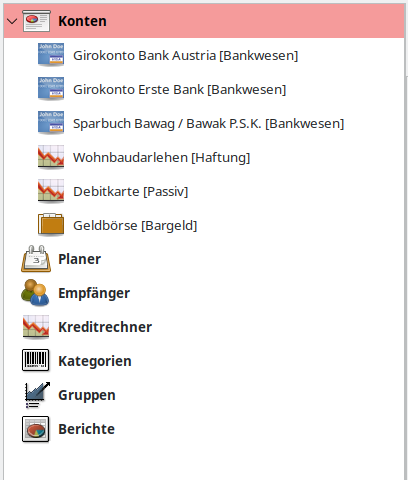
\includegraphics[width=0.28\textwidth]{image/screenshot/home_navigation}
\vspace{-5pt}						% space between the floating and the caption below the floating
\captionsetup{%						% for a change of options of the caption package
	format=plain,					% to avoid error message with labelsep option below, default=hang
	name=Abb.,						% rename label caption, default="Figure" (or "Table")
	justification=centering,		% centring of text and caption label 
	labelsep=newline				% define the separator between the label and the caption text
}
\caption{Navigationsbereich}		% \caption is mandatory to reference a figure in lof
\vspace{-40pt}						% space below the caption
\label{home_navigation}
\end{wrapfigure}

Im Navigationsbereich wird die Liste der Registerkarten in Fettdruck angezeigt:
	\begin{itemize}
		\item \menus{Konten}%Accounts},
		\item \menus{Planer}%Scheduler},
		\item \menus{Empfänger}%Payees},
		\item \menus{Kreditrechner}%Credits simulator},
		\item \menus{Kategorien}%Categories},
		\item \menus{Gruppen}%Budgetary lines},
		\item \menus{Berichte}%Reports}.
	\end{itemize}
Wenn Sie auf das kleine schwarze Dreieck links neben den Registerkarten \menus{Konten} oder \menus{Berichte} klicken, können Sie die Liste der Unterregisterkarten durchblättern oder aufrollen. Sie können die Reihenfolge der Registerkarten und Unterregisterkarten ändern, indem Sie auf eine von ihnen klicken und sie in der Liste nach oben oder unten ziehen.%By clicking on the small black triangle to the left of the  \menus{Accounts} or \menus{Reports} tabs,  you can scroll or roll up the list of their sub-tabs. You can change the order of tabs and sub-tabs by clicking on one of them and dragging it up or down the list.

\vspacepdf{5mm}

\textbf{Notiz}:  Je nach dem Thema der Desktop-Umgebung oder des Fenstermanagers, die Sie verwenden, können diese dreieckigen Symbole durch andere Zeichen wie +, -, >, < usw. ersetzt werden.%These triangles can be replaced, depending on the theme of the desktop environment or window manager you are using, by other characters such as +, -,>, <, and so on.

\vspacepdf{3mm}

Sie können eine dieser Registerkarten oder Unterregisterkarten auswählen, indem Sie auf ihren Namen klicken. Sie können die Auswahl in dieser Liste von Registerkarten und Unterregisterkarten auch mit den \keys{Pfeiltasten Hinauf}, \keys{Pfeiltasten Herunter}, \keys{Bild Hinauf} oder \keys{Bild Herunter} oder mit dem Mausrad verschieben (diese Option muss in den Voreinstellungen \vref{setup-display-toolbars} aktiviert werden).%You can select one of these tabs or sub-tabs by clicking on its name. You can also move the selection in this list of tabs and sub-tabs with the \key{Up Arrow}, \key{Down Arrow}, \key{Page Up} ou \key{Page Down} keys, or with the mouse wheel (option to be checked in the preferences \vref{setup-display-toolbars}). 

\vspacepdf{3mm}
Der Inhalt der Auswahl wird im Bereich details angezeigt.%The contents of the selection are displayed in the details panel.

\vspacepdf{3mm}

Sie können die Breite des Navigationsbereich verkleinern oder vergrößern, indem Sie auf den dünnen vertikalen Balken zwischen diesem Fenster und dem Bereich details klicken und ihn verschieben. Wenn die Breite des Fensters auf Null reduziert oder auf die maximale Breite des Grisbi-Fensters vergrößert wurde, kann sich die dünne vertikale Leiste links oder rechts vom Fenster befinden.  Suchen Sie diesen und schieben Sie ihn an die gewünschte Stelle zurück.%You can reduce or enlarge the width of the navigation panel by clicking on the thin vertical bar between this panel and the details panel, and moving it. If the width of the window has been reduced to zero, or enlarged to the maximum of the width of the Grisbi window, the thin vertical bar may be to the left or to the right of the window.  Locate this and slide it back to the desired location.

\vspacepdf{3mm}

Die \indexword{Kontextmenüs}\index{Kontextmenü}, die durch einen Rechtsklick mit der Maus zugänglich sind, sind auf den Elementen dieses Bereich verfügbar und bieten die folgenden Funktionen:%The \indexword{context menus}\index{context menus}, accessible by a right-click of the mouse, are available on the elements of this panel and offer the following functions:

\begin{itemize}
	 \item Auf \menus{Konten}%Accounts}:
		\begin{itemize}
			 \item \menus{Konto erstellen}%New account};
		\end{itemize}
	 \item Erfasste Konten:%On any account: 
		\begin{itemize}
			 \item \menus{Konto erstellen}%New account},
			 \item \menus{Konto löschen}%Remove this account};
		\end{itemize}
	 \item Auf \menus{Empfänger}%Payees}:
		\begin{itemize}
			 \item \menus{Empfänger erstellen}%New payee},
			 \item \menus{Den ausgewählten Empfänger löschen}%Delete selected payee},
			 \item \menus{Den ausgewählten Empfänger bearbeiten}%Edit selected payee},
			 \item \menus{Empfänger verwalten}%Manage payees},
			 \item \menus{Verwaiste löschen}%Remove unused payees};
		\end{itemize}
	 \item Auf \menus{Kategorien}%Categories}: 
		\begin{itemize}
			 \item \menus{Kategorie erstellen}%New category},
			 \item \menus{Die ausgewählten Kategorie löschen}%Delete selected category},
			 \item \menus{Die ausgewählte Kategorie bearbeiten}%Edit selected category},
			 \item \menus{Kategorien (*.csgb) importieren}%Import a file of categories (.csgb)},
			 \item \menus{Kategorien (*.csgb) exportieren}%Export the list of categories (.csgb)};
		\end{itemize}
	 \item Auf \menus{Gruppen}%Budgetary lines}:
		\begin{itemize}
			 \item \menus{Gruppe erstellen}%New budgetary line},
			 \item \menus{Die ausgewählten Gruppe löschen}%Delete selected budgetary line},
			 \item \menus{Die ausgewählte Gruppe bearbeiten}%Edit selected budgetary line},
			 \item \menus{Gruppen (*.isgb) importieren}%Import a file of budgetary lines (*.isgb)},
			 \item \menus{Gruppen (*.isgb) exportieren}%Export the list of budgetary lines (*.isgb)};
		\end{itemize}
	 \item Auf \menus{Berichte}: \menus{Bericht erstellen};%New report}%Report}: \menus{New report};
	 \item Auf Erfasste Berichte:%any report: 
		\begin{itemize}
			 \item \menus{Bericht erstellen}%New report},
			 \item \menus{Den ausgewählten Bericht löschen}%Remove this report}.
		\end{itemize}
\end{itemize}

\section{Bereich details\label{home-details}}

Das Bereich details zeigt alle Details zu den über die Informationsleiste oder das Navigationsbereich ausgewählten Registerkarten oder Unterregisterkarten an. Dies ist der Hauptarbeitsbereich von Grisbi.

Sie können es verkleinern oder vergrößern, indem Sie auf die dünne vertikale Leiste zwischen diesem Fenster und dem Navigationsbereich klicken und sie ziehen. Wenn die Breite dieses Fensters auf Null reduziert oder auf die maximale Breite des Grisbi-Fensters vergrößert wurde, kann sich die dünne vertikale Leiste links oder rechts vom Fenster befinden. Suchen Sie diesen und schieben Sie ihn an die gewünschte Stelle zurück.%The details panel displays all the details on the tabs or sub-tab selected by the Information bar or Navigation panel. This is the main work area of Grisbi.
%You can reduce or enlarge its width by clicking on the thin vertical bar between this window and the navigation panel, and dragging it. If the width of the this panel has been reduced to zero or enlarged to the maximum of the width of the Grisbi window, the thin vertical bar may be to the left or to the right of the window.  Locate this and slide it back to the desired location.

\begin{figure}[htbp]			% h=here, t=top, b=bottom, p=page of float to force the figure here, not in a next page.
	\begin{center}
		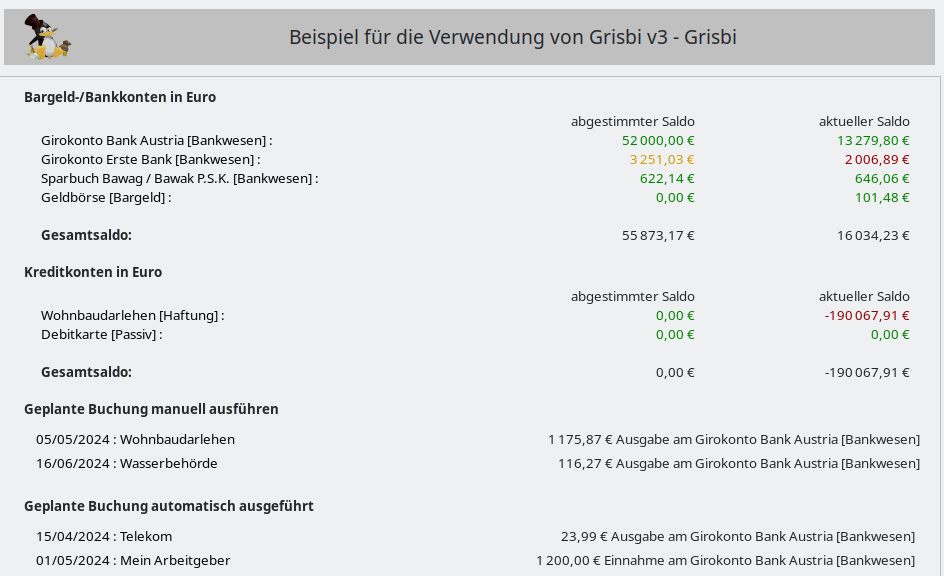
\includegraphics[width=1\textwidth]{image/screenshot/home_details.png}
	\end{center}
	\caption{Geändertes Bereich details}		% sous-titre/subtitle
	\label{home_details}
\end{figure}
 
\subsection{Anzeige von Details auf der Startseite\label{home-details-homepage}}

Wenn Sie die Registerkarte \menus{Konten} auswählen, wird das Bereich details angezeigt:%By selecting the \menus{Accounts} tab, the details panel displays:

\begin{itemize}
	\item in einem grauen Hintergrundbanner nach oben:%to the top in a grey background banner:
		\begin{itemize}
			\item das \menus{Grisbi}-Symbol (das ausgeblendet werden kann, siehe \vref{setup-display-logo-icon}),
			\item und auf der rechten Seite den \indexword{Titel}\index{Titelanzeige!Titel}\index{Hauptseite} der aktuell geladenen Buchhaltungsdatei in der Form \dequote{zugewiesener Name - Grisbi}; Sie können diese Bezeichnung unter drei Möglichkeiten im Menü \menus{Bearbeiten - Einstellungen} festlegen (siehe den Abschnitt \vref{setup-display-addresses-titles}, Adressen \& Bezeichnungen):%in a box on a gray background, on the left, the \menus{Grisbi} icon (which can be hidden, see \vref{setup-display-logo-icon}) and on the right the \indexword{title}\index{title display!title}\index{home page} of the accounts file you currently have loaded, in the form \enquote{assigned name - Grisbi}; you can define this label, from among three possibilities, in the \menus{Edit preferences} menu (see the paragraph \vref{setup-display-addresses-titles}):
				\begin{itemize}
			 		\item die \menus{Bezeichnung} (standardmäßig): Dies ist der Name, den Sie zur Identifizierung der Art des Kontos verwenden, z. B. \dequote{Meine Konten} oder \dequote{Business}, den Sie bei der Erstellung der Kontodatei eingegeben haben; Sie können ihn hier im Feld \menus{Bezeichnung} bearbeiten; dies kann nützlich sein, wenn Sie mehrere \indexword{Bezeichnungen}\index{Bezeichnung} verwalten,%the \menus{Accounting entity}: This is the name you use to identify the type of account e.g. \enquote{My Accounts} or \enquote{Business}, which you entered when the account file was created; you can edit it here in the \menus{Name of accounting entity} field; this can be useful if you manage multiple \indexword{accounting entities}\index{accounting entity}, 
					\item die \menus{Kontoinhaber}: den Namen des Inhabers (oder des Kontoverwalters) des zuletzt aufgerufenen Kontos; wenn der Inhaber nicht in den Kontoeigenschaften definiert ist, zeigt Grisbi den Namen dieses Kontos an,%the \menus{Account owner name}: the name of the owner (or  account manager) of the last account accessed; if the holder is not defined in the account properties, Grisbi displays the name of this account,
			 		\item die \menus{Dateiname}: Dies ist der Name der Datei im aktuellen Verzeichnis in der Form \file{Name\_deiner\_Datei.gsb};%the \menus{Filename}: this is the name of the file in the current directory, in the form \file{name\_of\_your\_file.gsb};
			 	\end{itemize}
		\end{itemize}
	\item im hellgrauen Hauptbereich unterhalb des Banners:%in the main light grey area below the banner:
	 	\begin{itemize}
	 		\item für jede Währung getrennt, für alle Konten und \indexword{Kontengruppen}\index{Kontengruppe}, unter den Bezeichnungen \menus{abgestimmter Saldo} und \menus{aktueller Saldo}:%for each currency separately, for all accounts and \indexword{groups of accounts}\index{groupe de comptes},  under the label \menus{Reconciled balance} and \menus{Current balance}:
				\begin{itemize}
					\item den Saldo der Bank- und Kassenkonten, den Teilsaldo der Kontengruppen und deren Gesamtsaldo,%the balance of the bank and cash accounts, the partial balance of the groups of accounts and their global balance,
					\newline
					\textbf{Notiz}: können Sie die Reihenfolge der Anzeige der Teilsalden der Kontengruppen anpassen (siehe Abschnitt \vref{setup-general-home-partBalance}, Teilweise Salden der Kontenliste)%you can adjust the display order of the partial balances of the account groups (see the section \vref{setup-general-home-partBalance}, \menus{Partial balances of the list of accounts}).			 
					\item der Saldo der Passivkonten und ihr Endsaldo,%the balance of the liability accounts and their final balance,
					\item der Saldo der Vermögenskonten und ihr Endsaldo;%the balance of the asset accounts and their final balance;
				\end{itemize}
			\item die \indexword{Warnungen vor automatisch geplanten Einträgen}\index{Warnung!geplanter Eintrag} mit ihrem Datum, entsprechend der im \menus{Bearbeiten - Einstellungen} getroffenen Auswahl (siehe den Abschnitt \vref{Einrichten - Allgemeiner Plan}, \menus{Planer}),%the \indexword{alerts from automatically scheduled entries}\index{alert!scheduled entry} with their date, wording and amount, according to the choices made in the \menus{Edit - Preferences} menu (see the section \vref{setup-general-planned}, \menus{Timetable});
			\item die Liste der Konten, deren Saldo unter den \menus{Mindestsaldo zulässig} gefallen ist,%the list of accounts whose balance has fallen below the \menus{Minimum authorized balance};
			\item die Liste der Konten, deren Saldo unter den \menus{Mindestsaldo festgelegt} gefallen ist.%the list of accounts whose balance has fallen below the \menus{Minimum desired balance}.
		\end{itemize}
\end{itemize}

\vspacepdf{5mm}

\textbf{Notiz}: Definitionen der Begriffe \menus{Mindestsaldo zulässig} und \menus{Mindestsaldo festgelegt} finden Sie im Abschnitt \vref{accounts-properties}, \menus{Konten bearbeiten}.%For definitions of \menus{Minimum authorized balance} and \menus{Minimum desired balance}, see the \vref{accounts-properties}, \menus{Account Properties} section.

\vspacepdf{3mm}

Die Kontobezeichnungen werden in \textcolor{black}{schwarz} angezeigt. Wenn Sie den Mauszeiger über eine dieser Zeilen bewegen, ändert sich ihre Farbe in \textcolor{gray}{grau}.%The account labels are displayed in \textcolor{black}{schwarz}; as the mouse cursor moves over the line of one of these, its colour changes to \textcolor{gray}{grau}.

Eine Balance, die größer ist als die \menus{Mindestsaldo festgelegt}, wird in \textcolor[RGB]{0,126,0}{grün} angezeigt: Wenn sich der Cursor über die Zeile bewegt, ändert sich ihre Farbe in \textcolor[RGB]{0,227,0}{hellgrün}.%A balance greater than the \menus{Minimum desired Balance} is displayed in \textcolor[RGB]{0,126,0}{green}: as the cursor moves over the line, its colour changes to \textcolor[RGB]{0,227,0}{light green}.

Ein Saldo, der kleiner als der {Mindestsaldo festgelegt} und größer als der {Mindestsaldo zulässig} ist, wird in \textcolor[RGB]{230,155,0}{orange} angezeigt: wenn der Zeiger auf seiner Linie vorbeigeht, ändert sich diese Farbe zu \textcolor[RGB]{255,200,0}{hellorange}.%A balance less than the \menus{Minimum desired balance} and greater than the \menus{Minimum authorized balance} is displayed in \textcolor[RGB]{230,155,0}{orange}: as the pointer passes on its line, this color changes to \textcolor[RGB]{255,200,0}{light orange}.

Ein Saldo, der kleiner ist als der {Mindestsaldo zulässig}, wird in \textcolor[RGB]{153,0,0}{Dunkelrot} angezeigt: wenn der Zeiger über die Linie fährt, ändert sich diese Farbe zu \textcolor{red}{red}.%A balance less than the  \menus{Minimum authorized Balance}  is displayed in \textcolor[RGB]{153,0,0}{dark red}: as the pointer passes over its line, this color changes to \textcolor{red}{red}.

Wenn Sie den Mauszeiger über die Zeile eines Kontos bewegen, zeigt jede Farbänderung an, dass die im markierten Konto enthaltenen Datensätze angezeigt werden, wenn Sie mit der Maus klicken (rechts oder links), als ob das Konto mit der Informationsleiste oder dem Navigationsbereich ausgewählt worden wäre.%When you move the mouse pointer over the line of an account, any color change indicates that if you click (right or left) with the mouse, the records contained in the highlighted account is displayed, as if the account had been selected with the information bar or navigation panel.

Ein Teilsaldo kann für eine Gruppe von Konten angegeben werden. Ist er definiert, wird er in \textcolor[RGB]{40,40,255}{dunkelblau} angezeigt (wie in der Abbildung \vref{home_details}). Wenn er negativ ist, kann er in \textcolor[RGB]{153,0,0}{dunkelrot} erscheinen (siehe \vref{setup-general-home-partBalance}, \menus{Teilsalden}). Eine Teilbilanzzeile ändert ihre Farbe nicht, wenn der Mauszeiger über ihr steht, da Sie die einzelnen Einträge einer Kontengruppe nicht sehen können.%A partial balance can be specified for a group of accounts  If defined this is displayed in \textcolor[RGB]{40,40,255}{dark blue} (see the example in the figure \vref{home_details}). If it is negative, it may appear in \textcolor[RGB]{153,0,0}{dark red}, (see  \vref{setup-general-home-partBalance}, \menus{Balances partials of the list of accounts}). A partial balance line does not change color when the mouse pointer is over it, because you can not view the individual entries for of an group of accounts.

% espace pour changement de thème
\vspacepdf{3mm}
Sie können bestimmte Aspekte der Anzeige des Bereich details konfigurieren:%You can configure certain aspects of the display of the details panel:
\begin{itemize}
	\item in the \menus{Bearbeiten - Einstellungen} menu: %TODO verify sections/paragraphs with \vref{setup-xxx}
	\begin{itemize}
		\item \menus{\indexword{Allgemein}\index{allgemein}}:
		\begin{itemize}
			\item \menus{Allgemeines}, tab \menus{Planer}\index{planer}: Abschnitt \vref{setup-general-planned};
			\item \menus{Startseite}:
			\begin{itemize}
				\item \menus{Berechnung der Salden}: Absatz \vref{setup-general-home-balance},
				\item \menus{Teilsalden}: Absatz \vref{setup-general-home-partBalance};
			\end{itemize}
		\end{itemize}
		\item \menus{\indexword{Anzeigeoptionen}\index{anzeigeoptionen}}:
		\begin{itemize}
			\item \menus{Schriften \& Logo}\index{Schriften}\index{logo}: Abschnitt \vref{setup-display-logo},
			\item \menus{Adressen \& Bezeichnungen}\index{bezeichnunge}\index{adresse}: Abschnitt \vref{setup-display-addresses-titles};
		\end{itemize}
	\end{itemize}
	\item auf der tab \menus{Eigenschaften} der einzelnen Konten in der Rubrik \menus{Saldoinformationen}:%in the \menus{Properties} tab of each account:
	\begin{itemize}
		\item Konten unterhalb des \menus{Mindestsaldo zulässig}\index{saldo!mindest zulässig}: Abschnitt \vref{accounts-properties}:
		\item Konten unterhalb des \menus{Mindestsaldo festgelegt}\index{saldo!mindest festgelegt}: Abschnitt  \vref{accounts-properties}.
	\end{itemize}
\end{itemize}

%In particular, if you find a spelling error in this page, you can correct it: see the paragraph \vref{setup-general-home-final}, \menus{?? Pluriel de final ??} !

\section{Menüleiste\label{home-menus}}

Wie in vielen Grafikanwendungen sind die meisten wichtigen Funktionen von Grisbi über die Menüs in der \indexword{Menüleiste}\index{Menüleiste} zugänglich. Die Funktionen werden im Folgenden detailliert beschrieben.%As in many graphics applications, most of Grisbi's important features are accessible through the menus in the \indexword{Menu Bar}\index{barre de menus}. The features are detailed below.


\subsection{Menü \menus{Datei}\label{home-menus-file}}

Dieses Menü enthält die folgenden Funktionen:%This menu includes the following functions:

\vspace{3mm}
\begin{itemize}[rightmargin=.6cm]
	\item \menus{Neues Fenster}: nicht funktionsfähig (vielleicht in Zukunft?)%TODO: to update
	%non-functional (perhaps in the future?)
\end{itemize}

\noindent
\begin{minipage}{.7\linewidth}
	\begin{itemize}[rightmargin=.6cm]
		\item \menus{Neu}: erstellt eine neue Grisbi-Datei mit der \gls{Dateinamenserweiterung} \file{.gsb}; die aktuelle Datei wird daher geschlossen und eine neue leere Datei mit einem leeren Konto erstellt (Tastenkombination \keys{Strg+N}), siehe den Abschnitt \vref{start-newfile}; nicht zu verwechseln mit der Erstellung eines neuen Kontos;%creates a new Grisbi file of \gls{extension}\file{.gsb}; the current file is therefore closed and a new empty file is created with an empty account (shortcut \keys{Ctrl+N}), see the section \vref{start-newfile}; not to be confused with the creation of a new account;%\menus{Nouveau fichier de comptes}: crée un nouveau fichier Grisbi d'\gls{extension} \file{.gsb}; le fichier courant est donc fermé et un nouveau fichier vide est créé avec un compte vide (raccourci-clavier \keys{Ctrl+N}), voir la section \vref{start-newfile}; à ne pas confondre avec la création d'un nouveau compte;	 
		\item \menus{Öffnen}: öffnet Ihren Dateimanager und ermöglicht es Ihnen, eine Kontodatei mit der \gls{Dateinamenserweiterung} \file{.gsb} zu suchen, auszuwählen und zu öffnen (Tastenkombination \keys{Strg+O}).%opens your file manager, allowing you to search for, select and open an account file with the \file{.gsb} \gls{extension} (shortcut \keys{Ctrl+O}).%ouvre votre gestionnaire de fichiers, permettant de rechercher, sélectionner et ouvrir un fichier de comptes d'\gls{extension} \file{.gsb} (raccourci-clavier \keys{Ctrl+O});
		\item \menus{Zuletzt geöffnete Dateien}: zeigt eine Liste der letzten n mit Grisbi geöffneten Dateien an (nur wenn mehr als eine geöffnet wurde); diese Anzahl ist im Menü \menus{Bearbeiten - Einstellungen} konfigurierbar, siehe Abschnitt \vref{setup-general-files-manage}, {Account Files Management}; %TODO to translate
		%displays a list of the last n files opened with Grisbi (only if more than one has been opened); this number is configurable in the menu \menus{Edit - Preferences}, see section \vref{setup-general-files-manage}, \menus{Account Files Management};%affiche la liste des n derniers fichiers ouverts avec Grisbi (seulement s'il y en a eu plusieurs); ce nombre est configurable dans le menu \menus{Edition - Préférences}, voir la section \vref{setup-general-files-manage}, \menus{Gestion des fichiers de compte};
	\end{itemize}
\end{minipage}
\hspace{10pt}	
\begin{minipage}{.3\linewidth}
	\vspace{-10pt}					% space above the floating (minus intextsep=separation between float and text in text)
	\centering						% centering the floating figure in the "wrap"
	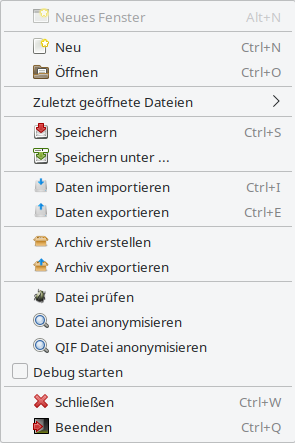
\includegraphics[width=1\textwidth]{image/screenshot/home_menubar_file}
	\vspace{-10pt}					% space between the floating and the caption below the floating
	\captionsetup{
		type=figure,%				% define "figure" or "table" type, mandatory
		name=Abb.,%					% rename label caption, default="Figure" (or "Table")
		labelsep=newline}			% define the separator between the label and the caption text
	\caption{Menü \menus{Datei}}	% \caption is mandatory to reference a figure in lof
	%\vspace{30pt}					% space below the caption
	\label{home_menubar_file}
\end{minipage}

\begin{itemize}
	\item \menus{Speichern}: Speichert Änderungen in der aktuellen Grisbi Datei (Tastenkombination \keys{Ctrl+S});%\menus{Save}: Saves the current account file (shortcut \keys{Ctrl+S});%\menus{Enregistrer}: enregistre le fichier de comptes en cours (raccourci-clavier \keys{Ctrl+S});
	\item \menus{Speichern unter ...}: Öffnet einen Dateimanager, um die Datei der aktuellen Konten unter einem Namen und an einem Ort Ihrer Wahl zu speichern; Grisbi verwendet standardmäßig das aktuelle Verzeichnis, den Namen der Datei der aktuellen Konten und die \gls{Dateinamenserweiterung} \file{.gsb};%\menus{Save As}: opens a file manager to save the current accounts file with the name and location of your choice; Grisbi defaults to the current directory, the name of the current accounts file, with the \file{.gsb} extension;%\menus{Enregistrer sous}: ouvre un gestionnaire de fichiers pour enregistrer le fichier de comptes en cours avec le nom et à l'emplacement de votre choix; Grisbi vous propose par défaut le répertoire courant, le nom du fichier de comptes en cours, avec l'\gls{extension} \file{.gsb};
	\item \menus{Daten importieren}: Startet den Assistent \dequote{Daten importieren} einer anderen Software (Tastenkombination \keys{Strg+I}); Sehen \vref{move-import-importinit}%\menus{Import file...}: starts the \enquote{Importing transactions into Grisbi} wizard of another software (shortcut \keys{Ctrl+I}); see \vref{move-import-importinit};%\menus{Importer un fichier}: démarre l'assistant d'importation de fichiers d'un autre logiciel (raccourci-clavier \keys{Ctrl+I}); voir la section \vref{move-import-importinit};
	\item \menus{Daten exportieren}: Startet den Assistent \dequote{Konten exportieren} (Tastenkombination \keys{Strg+E}); Sehen \vref{move-export};%\menus{Export accounts as QIF/CSV file}: starts the \enquote{Exporting Grisbi accounts} wizard (shortcut \keys{Ctrl+E}); see \vref{move-export};%\menus{Exporter vers un fichier QIF/CSV}: démarre l'assistant d'exportation de fichiers de compte (raccourci-clavier \keys{Ctrl+E}); voir la section \vref{move-export};	
	\item \menus{Archiv erstellen}: Startet den Assistent Archive erstellen; Sehen \vref{datamanagement-history-new};%\menus{Archive transactions}: starts the archive creation wizard; see \vref{datamanagement-history-new};%\menus{Créer une archive}: démarre l'assistant de création d'archive; voir la section \vref{datamanagement-history-new};	
	\item \menus{Archiv exportieren}: Startet den Assistent Archive exportieren; Sehen \vref{datamanagement-history-export};%\menus{Export an archive as GSB/QIF/CSV file}: starts the archive export wizard; see \vref{datamanagement-history-export};%\menus{Exporter une archive vers un fichier GSB/QIF/CSV}: démarre l'assistant d'exportation d'archive; voir la section \vref{datamanagement-history-export};
	\item \menus{Datei prüfen}: Startet den Assistent Konsistenzprüfung, die Ihnen helfen wird, nach Unstimmigkeiten in Ihrer Kontodatei zu suchen; Sehen \vref{maintenance-file-debug}%\menus{Debug account file}: starts the debug wizard for this file, which will help you look for inconsistencies in your account file; see \vref{maintenance-file-debug};%\menus{Déboguer le fichier de comptes}: démarre l'assistant de débogage de ce fichier, qui va vous aider à chercher des incohérences dans votre fichier de comptes; voir la section \vref{maintenance-file-debug};
	\item \menus{Datei anonymisieren}: Startet den Assistent \dequote{Grisbi Datei anonymisieren}, der eine anonyme Kopie Ihrer Kontodatei erstellt; diese Datei kann an einen Fehlerbericht angehängt werden;%\menus{Obfuscate account file}: starts the wizard that produces an anonymous copy of your account file; this file can be attached to a bug report; see \vref{maintenance-file-anonymous};%\menus{Rendre anonyme le fichier de comptes}: démarre l'assistant qui produit une copie anonymée (de manière irréversible) de votre fichier de comptes; ce fichier pourra être joint à un rapport de bogue; voir la section \vref{maintenance-file-anonymous};	
	\item \menus{\gls{QIF} Datei anonymisieren}: Startet den Assistent QIF Datei anonymisieren, der eine anonyme Kopie dieser Datei erstellt; diese Datei kann an einen Fehlerbericht angehängt werden; Sehen \vref{maintenance-QIF-anonymous};%\menus{Obfuscate QIF file}: starts the wizard that produces an anonymous copy of this file; this file can be attached to a bug report; see \vref{maintenance-QIF-anonymous};%\menus{Rendre anonyme le fichier QIF}: démarre l'assistant qui produit une copie anonymée (de manière irréversible) de ce fichier; ce fichier pourra être joint à un rapport de bogue; voir la section \vref{maintenance-QIF-anonymous};	
	\item \menus{Debug starten}: Aktiviert den Debug Modus, der eine Protokolldatei der Ereignisse erstellt; Sehen \vref{maintenance-debug-mode} %\menus{Debug mode}: puts Grisbi in debug mode, which creates a log file of events; see \vref{maintenance-debug-mode};%\menus{Mode de débogage}: met Grisbi en mode de débogage, qui crée un fichier-journal des évènements; voir la section \vref{maintenance-debug-mode}; 	
	\item \menus{Schließen}: Schließt die aktuell geöffnete Grisbi Datei; Grisbi bietet Ihnen an, sie zu speichern, falls Sie dies noch nicht getan haben (Tastenkombination \keys{Strg+W}). %\menus{Close}: closes the current accounts file; Grisbi offers to save it if you have not already done it (shortcut \keys{Ctrl+W});%\menus{Fermer}: ferme le fichier de comptes en cours; Grisbi vous propose de l'enregistrer si ce n'est déjà fait (raccourci-clavier \keys{Ctrl+W});
	\item \menus{Beenden}: Beendet Grisbi; Grisbi wird Sie zunächst auffordern, die Kontendatei zu speichern, falls Sie dies noch nicht getan haben (Tastenkombination \keys{Strg+Q}).%\menus{Quit}: close Grisbi; Grisbi will first ask you to save the accounts file, if you have not already done so (shortcut \keys{Ctrl+Q});%\menus{Quitter}: ferme Grisbi; Grisbi vous propose auparavant d'enregistrer le fichier de comptes, si ce n'est pas déjà fait (raccourci-clavier \keys{Ctrl+Q}).
\end{itemize}


\subsection{Menü \menus{Bearbeiten}\label{home-menus-edit}}

\textbf{Notiz}: Im Menü Bearbeiten sind einige Einträge erst aktiv wenn ein Konto oder eine Buchung ausgewählt wird.

Dieses Menü enthält die folgenden Funktionen:%This menu includes the following functions:

\vspace{3mm}
\noindent
\begin{minipage}{.7\linewidth}
	\begin{itemize}[rightmargin=.6cm]
		\item \menus{Buchung bearbeiten}: ermöglicht es, einen ausgewählten Vorgang zu korrigieren, siehe Abschnitt \vref{transactions-modify}, \menus{Modification d'une opération};%TODO to translate
		% allows a selected operation to be rectified, see section \vref{transactions-modify}, \menus{Modification d'une opération};%TODO to translate
		%\menus{Éditer l'opération}: permet la rectification d'une opération existante, voir la section \vref{transactions-modify}, \menus{Modification d'une opération};
		\item \menus{Buchung erstellen}: ermöglicht die Erstellung einer neuen Transaktion in einem Konto (Tastaturkürzel \keys{Strg+T}), siehe den Abschnitt \vref{transactions-new}, \menus{Saisie d'une nouvelle opération};%TODO to translate
		% allows the creation of a new transaction in an account (shortcut \keys{Ctrl+T}), see the section \vref{transactions-new}, \menus{Saisie d'une nouvelle opération};%TODO to translate
		%\menus{Nouvelle opération}: permet la création d'une nouvelle opération dans un compte (raccourci-clavier \keys{Ctrl+T}), voir la section \vref{transactions-new}, \menus{Saisie d'une nouvelle opération};
		\item \menus{Buchung löschen}: löscht einen ausgewählten Vorgang, siehe Abschnitt \vref{transactions-delete}, \menus{Deleting a transaction};%TODO to translate
		% deletes a selected operation, see section \vref{transactions-delete}, \menus{Deleting a transaction};
		%\menus{Supprimer une opération}: supprime une opération existante, voir la section \vref{transactions-delete}, \menus{Suppression d'une opération};
	\end{itemize}
\end{minipage}
\hspace{10pt}	
\begin{minipage}{.3\linewidth}
	\vspace{-5pt}					% space above the floating (minus intextsep=separation between float and text in text)
	\centering						% centering the floating figure in the "wrap"
	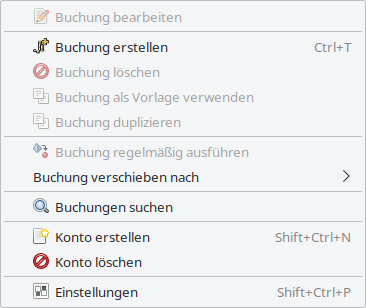
\includegraphics[width=1\textwidth]{image/screenshot/home_menubar_edit}
	\vspace{-15pt}					% space between the floating and the caption below the floating
	\captionsetup{
		type=figure,%				% define "figure" or "table" type, mandatory
		name=Abb.,%					% rename label caption, default="Figure" (or "Table")
		labelsep=newline}			% define the separator between the label and the caption text
	\caption{Menü \menus{Bearbeiten}}	% \caption is mandatory to reference a figure in lof
	%\vspace{30pt}					% space below the caption
	\label{home_menubar_edit}
\end{minipage}

\begin{itemize}
	\item \menus{Buchung als Vorlage verwenden}: Erstellt die Kopie eines ausgewählten Vorgangs, wobei das aktuelle Datum in das Buchungsformular eingetragen wird, siehe Abschnitt \vref{transactions-model}, \menus{Opération sélectionnée comme modèle};%TODO to translate
	%Use selected transaction as a template}: allows you to create a new operation from a selected operation, see \vref{transactions-model}, \menus{Selecting a transaction for use as a template}:
	%\menus{Utiliser l'opération sélectionnée comme modèle}: permet de créer une nouvelle opération à partir d'une opération sélectionnée, voir la section \vref{transactions-model}, \menus{Opération sélectionnée comme modèle};
	\item \menus{Buchung duplizieren}: Erstellt eine Kopie, die mit dem ausgewählten Buchung identisch ist, und öffnet das Buchungsformular, siehe Abschnitt \vref{transactions-duplicate}, \menus{Clone a transaction};%TODO to translate
	%\item \menus{Clone transaction}: is used to duplicate an existing operation, see section \vref{transactions-duplicate}, \menus{Clone a transaction};
	%\menus{Cloner l'opération}: permet de dupliquer une opération existante, voir la section \vref{transactions-duplicate}, \menus{Clonage d'une opération};
	\item \menus{Buchung regelmäßig ausführen}: siehe Abschnitt \vref{transactions-schedule}, \menus{Converting a transaction to a scheduled transaction};%TODO to translate
	%\item \menus{Convert to scheduled transaction}: see section \vref{transactions-schedule}, \menus{Converting a transaction to a scheduled transaction};
	%\menus{Convertir en opération planifiée}: voir la section \vref{transactions-schedule}, \menus{Conversion d'une opération en opération planifiée};
	\item \menus{Buchung verschieben nach}: Verschiebt die Buchung auf das ausgewählte Konto, siehe Abschnitt \menus{Moving a transaction to another account};%TODO to translate
	%\item \menus{Move transaction to another account}: see section \vref{transactions-move}, \menus{Moving a transaction to another account};
	%\menus{Déplacer l'opération vers un autre compte}: voir la section \vref{transactions-move}, \menus{Déplacement d'une opération vers un autre compte};
	\item \menus{Buchungen suchen}:
	\begin{itemize}
		\item Öffnet die Suche nach Buchungen mit der Funktionalität von Berichte wenn eine Registerkarte des Navigationsbereich ausgewählt ist, siehe Abschnitt \vref{reports-creation}, \menus{Création d'un état}>>>;%TODO to modify
		%opens the properties window for a report when a navigation panel tab is selected, <<<see chapter \vref{reports-creation}, \menus{Création d'un état}>>>;%TODO to modify
		%ouvre la fenêtre de propriétés d'un état quand un onglet du panneau de navigation est sélectionné, voir le chapitre \vref{reports-creation}, \menus{Création d'un état};
		\item Zeigt das Suchfeld an, wenn ein Konto oder eine Buchung ausgewählt wird, siehe Abschnitt <<<\vref{accounts-search}, \menus{alphanumerische Suche?}>>> TO CREATE; %TODO to create
		%displays the search box when an account or transaction is selected, <<<see chapter \vref{accounts-search}, \menus{alphanumeric search}>>> TO CREATE; %TODO to create
		%affiche la fenêtre de recherche quand un compte ou une opération est sélectionné, <<<voir le chapitre \vref{accounts-search}, \menus{Recherche alphanumérique}>>> A CRÉER; %TODO to create
	\end{itemize}
	\item \menus{Konto erstellen}: Startet den Assistent Konto erstellen für die Erstellung eines neuen Kontos in Ihrer Grisbi-Datei (Tastaturkürzel \keys{Shift+Ctrl+N}), siehe Abschnitt \vref{accounts-new}, \menus{Creating a new account};%TODO to translate
	%\item \menus{New account}: starts the wizard for creating a new account in your Grisbi file (shortcut \keys{Shift+Ctrl+N}), see section \vref{accounts-new}, \menus{Creating a new account};
	%\menus{Nouveau compte}: démarre l'assistant de	création d'un nouveau compte dans votre fichier Grisbi (raccourci-clavier \keys{Maj \shift+Ctrl+N}), voir la section \vref{accounts-new}, \menus{Création d'un nouveau compte};
	\item \menus{Konto löschen}: löscht das ausgewählte Konto aus Ihrer Grisbi-Datei, siehe Abschnitt \vref{accounts-delete}, \menus{Removing the current account};%TODO to translate
	%\item \menus{Remove current account}: deletes the selected account from your Grisbi file, see section \vref{accounts-delete}, \menus{Removing the current account}:
	%\menus{Supprimer le compte courant}: efface le compte sélectionné de votre fichier Grisbi, voir la section \vref{accounts-delete}, \menus{Suppression d'un compte};
	\item \menus{Einstellungen}: ermöglicht die Konfiguration von Grisbi (Tastenkürzel \keys{Maj \shift+Strg+P}); siehe Kapitel \vref{setup}, \menus{Configuration of Grisbi}.%TODO to translate
	%\item \menus{Preferences}: allows you to configure Grisbi (shortcut \keys{Maj \shift+Ctrl+P}); see the chapter \vref{setup}, \menus{Configuration of Grisbi}.
	%\menus{Préférences}: permet de configurer Grisbi (raccourci-clavier \keys{Maj \shift+Ctrl+P}); voir le chapitre \vref{setup}, \menus{Configuration de Grisbi}.
\end{itemize}


\subsection{Menü \menus{Ansicht}\label{home-menus-display}}

\textbf{Notiz}: Im Menü \menus{Ansicht} sind die Einträge erst aktiv wenn ein Konto ausgewählt wird.%in the \menus{View} menu, entries are only active when an account is selected.

Dieses Menü enthält die folgenden Funktionen:%This menu includes the following functions: 
%TODO following
\vspace{3mm}
\noindent
\begin{minipage}{.7\linewidth}
	\begin{itemize}[rightmargin=.6cm]
	\item \menus{Show transaction form}: expands the Transaction/Scheduled form for the selected account;
	%Montrer le formulaire de saisie des opérations}: permet de développer le formulaire de saisie des opérations du compte sélectionné;
	\item \menus{Show reconciled}: displays reconciled transactions for the selected account (shortcut \keys{Alt+R});
	%Montrer les opérations rapprochées}: permet l'affichage des opérations rapprochées du compte sélectionné (raccourci-clavier \keys{Alt+R});
	\item \menus{Show lines archives}: displays the archive lines for the selected account (shortcut \keys{Alt+L});
	%Montrer les lignes d'archives}: affiche les lignes d'archives du compte sélectionné (raccourci-clavier \keys{Alt+L});
	\item \menus{Show \indexword{closed accounts}}\index{closed!account}: displays account(s) that have been closed and not deleted, see section \vref{accounts-properties}, \menus{Account properties?}; %TODO to update
	%\menus{Montrer les \indexword{comptes clos}}\index{compte!clos}: affiche le(s) compte(s) clos et non supprimé(s), voir la section \vref{accounts-properties}, \menus{Propriétés d'un compte};
	\end{itemize}
\end{minipage}
\hspace{10pt}	
\begin{minipage}{.3\linewidth}
	%\vspace{-10pt}					% space above the floating (minus intextsep=separation between float and text in text)
	\centering						% centering the floating figure in the "wrap"
	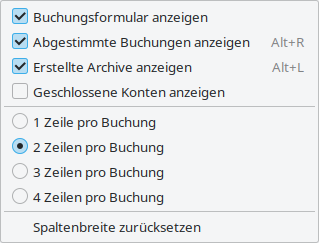
\includegraphics[width=1\textwidth]{image/screenshot/home_menubar_view}
	\vspace{-20pt}					% space between the floating and the caption below the floating
	\captionsetup{
	type=figure,%				% define "figure" or "table" type, mandatory
	name=Fig.,%					% rename label caption, default="Figure" (or "Table")
	labelsep=newline}			% define the separator between the label and the caption text
	\caption{\menus{View} Menu}		% \caption is mandatory to reference a figure in lof
	%\vspace{30pt}					% space below the caption
	\label{home_menubar_view}
\end{minipage}
\vspace{2mm}
\begin{addmargin*}[0pt]{.7cm} 	% modify margin, * : left = right, [] = obligatory argument indentation, {} = optional argument left indentation 
The following four functions can be used to configure the display of transactions for the selected account:
%Les quatres fonctions suivantes permettent de configurer l'affichage des opérations du compte sélectionné:
\end{addmargin*}
\vspace{-2mm}
\begin{itemize}
	\item \menus{Show one line per transaction}%Montrer une ligne par opération};
	\item \menus{Show two lines per transaction}%Montrer deux lignes par opération};
	\item \menus{Show three lines per transaction}%Montrer trois lignes par opération};
	\item \menus{Show four lines per transaction}%Montrer quatre lignes par opération};
	\vspace{2mm}
	\begin{addmargin}[0pt]{-.35cm} 	% modify margin, * : left = right, [] = obligatory argument indentation, {} = optional argument left indentation 
	And finally, the last function in the view menu:%Et enfin la dernière fonction du menu d'affichage:
	\end{addmargin}	
	\item \menus{Reset the column width}: allows you to reset the columns of the tranaction lists to their original width. 
	%Réinitialiser la largeur des colonnes}: permet de remettre les colonnes des listes d'opérations du compte sélectionné ou de l'échéancier à leur largeur d'origine.
\end{itemize}


\subsection{\menus{Help} menu\label{home-menus-help}}

Most of the choices in this menu give links to websites. In order for these links to work, you must have specified to Grisbi the navigation software (or browser) that you wish to use, in the \menus{Edit - Preferences} (see \vref{setup-general-programs}, \menus{Programmes}). The \menus{Help} menu includes the following choices\footnote{\strong{Translators Note:} A "help us with translation" menu item is mentioned in the French version of the manual but does note appear in the English version of Grisbi at release 1.0}:

\begin{itemize}
	\item \menus{Manual}: opens your browser to the  \dequote{Grisbi User Manual page} (shortcut key  \key{Ctrl}\key{H});
	\item \menus{Quick start}: opens your browser to the  \dequote{Grisbi Quick Start page};
%	\item \menus{Traduction}: opens your browser to the \dequote{Translate Grisbi}, to help us to widen the internationalization of Grisbi;
	\item \menus{About Grisbi...}: displays the program information box: you will find details about the version, the link to Grisbi's site, the acknowledgements page (contributors to the project) and the user license;
	\item \menus{Grisbi website}: opens your browser to the \lang{Grisbi}\footnote{\urlGrisbi{}} web site;
	\item \menus{Report a bug}: opens your browser to the \lang{Grisbi Bug Tracker page}\footnote{\urlBugTracker{}} to allow you to report a bug that you have discovered. You can also follow on this page the evolution of the corrections made to the reported bugs;
	\item \menus{Tip of the day}: opens a dialog box that displays a tip of use, different each time Grisbi starts; you can successively display all the tips, and choose whether or not the display of the tip of the day when starting Grisbi. To remove or reactivate the tip of the day, see \vref{setup-display-messages-trick}, \menus{Tip of the day}.
\end{itemize}


\section{Shortcut keys\label{home-shortcuts}}


Keyboard shortcuts make it easy to enter data and navigate through Grisbi's windows, avoiding the need to move and click. By using the ones corresponding to the most common manipulations for you, you improve your \indexword{ergonomics}\index{ergonomie} by limiting the important movements of your arms.
 
Grisbi has a number of keyboard shortcuts, presented here according to different themes (see also  \vref{introduction-manual-conventions}, \menus{Typographical conventions in this manual}).
.

\subsection{Application and files}

\begin{itemize}
	\item New accounts file: \key{Ctrl}\key{N}
	\item Open an account file: \key{Ctrl}\key{O}
	\item Register the account file: \key{Ctrl}\key{S}
	\item Close the account file: \key{Ctrl}\key{W}
	\item Close Grisbi: \key{Ctrl}\key{Q}
\end{itemize}


\subsection{Navigation panel}

\begin{itemize}
	\item Select a tab or account: \key{ Arrow Up}, \key{Arrow Down}, \key{Page Up} ou \key{Page Down}
\end{itemize}

\subsection{List of transactions and scheduled transactions}

\begin{itemize}
	\item Select a transaction: \key{Enter}
	\item Move selection:\key{Arrow Up} ou \key{Arrow Down}
	\item New transaction:  \key{Enter} on empty line, or \key{Ctrl}\key{T}
	\item Modify an transaction: \key{Enter}
	\item Delete an transaction: \key{Delete};
	\item Select a transaction for a reconciliation:\key{Ctrl}\key{P}
	\item Remove a reconciled transaction: \key{Ctrl}\key{R}
	\item Show or hide archival lines: \key{Altl}\key{L}
\end{itemize}


\subsection{Entry form}

\begin{itemize}
	\item The \key{Enter} is configurable: it can be set to either move in the input form, or to validate the entry
	\item Move to the next field: \key{Tab} (depending on your configuration choice)
	\item Cancel the current entry: \key{Esc}
	\item Accept auto-complete: \key{Tab} or \key{Enter} (depending on your configuration choice)
	\item  Euro symbol: \key{AltGr}\key{e}
\end{itemize}

\subsection{Drop down lists}

\begin{itemize}
	 \item Open a list: \key{Page Down} or \key{Down Arrow}
	 \item Move in the list: \key{Up Arrow}, \key{Down Arrow}, \key{Page Up} or \key{Page Down}
	 \item Validate a choice within a list: \key{Enter}
	 \item Currencies, ??exercises?? and methods of payment:
		\begin{itemize}
			\item open list: \key{Space}; 
			\item move in the list: \key{Up Arrow} or \key{Down Arrow};
			\item validate the item in the list: \key{Space}.
		\end{itemize}
\end{itemize}


\subsection{Dates entered on the calendar}

\begin{itemize}
	\item Opens a calendar (on the date field): \key{Ctrl}\key{Enter}
	\item Closes the calendar without changing the date: \key{Esc}
	\item Validate the selected date: \key{Enter}
	\item Next or previous day: \key{+} or \key{-}, \key{Right Arrow} or \key{Left Arrow}
	\item Previous or next week: \key{Up Arrow} or \key{Down Arrow}
	\item Previous or next month: \key{Page Up} or \key{Page Down}
	\item First day or last day of the month: \key{Start} or \key{End}
\end{itemize}


\subsection{Dates entered on keyboard }

\begin{itemize}
	\item Next or previous day: \key{+} or \key{-}
	\item Previous or next week: \key{Shift} \key{+} or \key{Majuscule} \key{-}
	\item Previous or next month: \key{Page Up} or \key{Page Down}
	\item Previous or Next Year: \key{Shift} \key{Page Up} or \key{Shift} \key{Page Down}
	\item Validate the selected date \key{Enter}
\end{itemize}


\subsection{Payees, categories, budget allocations, credit simulator, historical data and forecasts}

\begin{itemize}
	\item Move selection: \key{Up Arrow}, \key{Down Arrow}, \key{Page Up} or \key{Page Down}
%Ces raccourcis ne fonctionnent plus:
%	\item afficher les sous-catégories ou sous-imputations budgétaires (sur une catégorie ou une imputation budgétaire): \key{Espace};
%	\item afficher les opérations des sous-catégories ou sous-imputations budgétaires (sur une sous-catégorie ou une sous-imputation budgétaire): \key{Espace}.
\end{itemize}


\subsection{States and Configuration}

\begin{itemize}
	\item Select another tab: \key{Up Arrow}, \key{Down Arrow}, \key{Page Up}, \key{Page Down}
	\item Navigate between the tab panel and the different options in the settings panel: \key{Tab}, \key{Up Arrow}, \key{Down Arrow}, \key{Left Arrow} and \key{Right Arrow}
\end{itemize}

\subsection{Help}

\begin{itemize}
	\item Open your browser on the Grisbi User Manual page \key{Ctrl}\key{H}
\end{itemize}













